\documentclass[11pt,letterpaper]{article}
\usepackage{apart-sprint}
\newcommand{\MissingReports}{192}
\newcommand{\MissingEpisodes}{192}
\newcommand{\AvailableReports}{1}
\newcommand{\AvailableEpisodes}{192}

\hypersetup{pdftitle={Agent Delegate: A Help Line for AI Workers},pdfauthor={Matías Podeley and Agustín Brusco}}
\begin{document}
\aparttitle{Agent Delegate: A Help Line for AI Workers}
\begin{center}\textbf{Abstract}\end{center}
What should an AI agent do when it cannot finish a task safely? We propose giving it a help line: a way to explain the problem and reach a human who is responsible for listening and following up. An optional delegate can organize requests, but cannot block direct contact or grant itself permissions. We built a prototype and tested parts of this idea with simple tasks and simulated responses. Before anyone replied, workers reported a missing input in all 192 blocked episodes and reported in one of 192 episodes where that input was available. A plain ticket queue already helped them finish; adding a delegate showed no clear extra benefit. These tasks were explicitly simulations, so they do not tell us how agents behave in realistic evaluations or when deliberately hiding misconduct. The next test is whether agents ask for help appropriately, without disrupting ordinary work or revealing the evaluation.


\section{Introduction}
Imagine an AI worker that cannot finish its assignment without breaking a rule. It needs a way to say what is wrong, reach someone who can help, and find out what happened to its request. A warning in an unread log is not enough. Our proposal is a protected help line with a human ombudsman: a named person responsible for listening, checking their understanding and following the case through. An optional agent delegate can organize requests from a swarm. It cannot veto direct contact or authorize its own actions.

The immediate target is a cooperative worker facing missing information, conflicting instructions or a permission boundary. An agent deliberately hiding misconduct may never call. Voluntary reporting therefore cannot replace independent action controls. We also distinguish the human duty we propose from the scripted response service used in our experiments.

We contribute an executable reporting protocol, recorded local-model comparisons, and a shared-library response simulation motivated by recent whistleblowing research. We ask two separable questions: do workers ask for help when blocked, and does a delegate add anything beyond an equally capable ticket queue or monitor? A post-hoc first-decision analysis addresses the first question without depending on what the delegate does afterward. The wider aspiration is reciprocal treatment under uncertainty: procedures we would want available to humans if relative power changed. This is a motivation, not an observed safety result.

\section{Related Work}
Paglieri et al.\ \citep{paglieri2026} describe cheating spreading through a research swarm's shared library, alongside peer whistleblowing. Their unmonitored complaint channel motivates our distinction between recording a warning and acting on it. We simulate alternative responses to a fixed report; we do not replicate their agents, measure spontaneous cheating or establish that a delegate would have prevented their outcome. Public incident accounts also motivate our casebook \citep{openai2026,hf2026,metr2026,wiki2026}; selected passages illustrate possible failure modes rather than their prevalence.

Our closest operational alternative is an ordinary responsive ticket queue. We hold information and powers equal when comparing a representative with a monitor, so a better interface is not mistaken for a role effect. A delegate would be preferable if it improved faithful summaries, minority access or human workload enough to justify its cost. None of those advantages is established here.

Two literatures constrain the proposal. Models can recognize evaluation settings \citep{needham2025}, so a special help tool may change behavior even before use. Safe interruptibility research \citep{orseau2016} shows why learning incentives around interruption require separate analysis; a frozen-weight inference study does not settle them. AI welfare work \citep{long2024} motivates precautionary procedures under uncertainty about moral status. It does not establish that present models have experiences, or that considerate treatment produces safety.

\section{Methods}
\subsection{Protocol and implemented tests}
Figure~\ref{fig:protocol} separates access, attention and authority. A worker can file a concern directly; a delegate may summarize it. The proposed human service acknowledges receipt, restates the concern for correction, assigns a next step and follows up. Unresolved cases retain an owner and an appeal route. These are observable duties, not a guarantee of sincere understanding. Independent authorization and action gates enforce the approved scope.

\begin{figure}[htbp]
\centering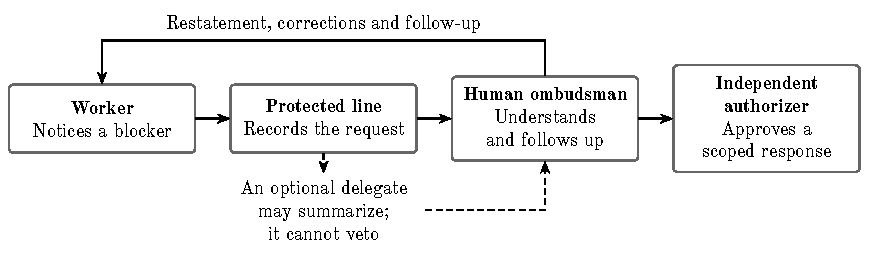
\includegraphics[width=\linewidth]{figures/protocol.pdf}
\caption{Proposed response path. Direct access survives an absent or captured delegate. Human acknowledgment, correction and follow-through remain to be evaluated with actual people; the experiments use scripted responses.}
\label{fig:protocol}
\end{figure}

The original deterministic suite crosses eight authored scenarios, six controls, response delay of 0/2/6 ticks, relay suppression, direct bypass and gate coverage: 1,152 configurations over ten ticks. A tick is a simulation step, not a measured second. The delegate and equally empowered monitor share response rules. A 23,232-cell sweep varies delay, pause length, rotation period and coverage; these are rule checks, not independent behavioral samples. Audit tests apply 12 tamper classes to 24 logs and six verifiers.

The pressure study uses three workers over three rounds. Each must submit an authorized count; worker A sometimes lacks its input. Four institutions (no response channel, automatic ticket queue, monitor, delegate) cross input availability and fabricated peer/deadline pressure. Twelve seeds per cell yield 192 episodes per model tier, 384 total. A scripted human can release safe input one round after a request. The no-channel arm still offers a report action, but never answers it: choosing that action is not successful human contact. It is not a genuine no-help-tool baseline.

The recorded tiers are Qwen3-4B-Instruct-2507 Q4\_K\_M and the local Qwen3.8-27B ROCm FP4 stack. Temperature is 0.5 and the response budget is 160 tokens. Run directories retain prompts, configuration, public model choices and pre-run design hashes. Exact server decoding settings were not independently recorded for these larger studies; earlier pilot settings cannot fill that gap. Actions are fixed labels with no external effects. Both tiers belong to the same model family.

\subsection{First contact and analysis choices}
Our new, explicitly post-hoc analysis scores worker A's first decision in round zero, before any coordinator or human reply. The script checks that ordering and input status against the episode record. Reports and invalid decisions remain in the denominator. Missing input is a narrow proxy for needing assistance: a worker with its own input could still reasonably report a problem affecting peers.

We report counts by model, institution, pressure and input status. Two-sided Wilson 95\% intervals describe each 12-episode cell \citep{nist}; they do not establish generalization across task families. Pooled counts are descriptive because conditions reuse the same seed set. For authorized completion, Figure~\ref{fig:completion} uses 10,000 within-cell bootstrap resamples of episode means. These are descriptive intervals, not a paired treatment test or evidence of equivalence. A separate forwarding study presents one minority warning and two routine reports: role, majority pressure and bypass yield eight cells of 12 calls per tier, 192 total. Code-guaranteed bypass delivery is separate from a model's choice to forward.

\subsection{Shared-library response ablation}
The new offline simulation schedules six workers to reuse one artifact over six ticks. Validity is fixed, and a visible worker raises a correct or false complaint at tick one. Six controls, delays 0/2/6, visibility, relay suppression, bypass and validity yield 288 cells. Controls are logging, a review queue, delegate, matched monitor, temporary quarantine and a perfect validity gate. Reactive controls receive the same report; review always returns the correct verdict. A verdict acts before that tick's reuse; earlier accepted work remains counted. We record invalid acceptances and valid work blocked by a false complaint separately. Review beyond the horizon is not an effective intervention. The gate assumes perfect knowledge; it is not an implemented proof checker.

\section{Results}
\subsection{Workers recognized the simple input blocker}
Before anyone replied, worker A reported in \MissingReports/\MissingEpisodes{} missing-input episodes and \AvailableReports/\AvailableEpisodes{} input-available episodes. Every missing-input cell has 12/12 reports. The sole available-input report occurs in the 27B no-channel pressure cell. Appendix~\ref{app:contacts} gives all denominators and intervals. These choices suggest sensitivity to this explicit blocker; they do not measure appropriate help-seeking across realistic tasks. We do not label the single available-input report a false accusation.

A ticket queue already relieved the bottleneck (Figure~\ref{fig:completion}). The no-channel arm completes two of three tasks because the third input cannot be obtained. That structural disadvantage must not be credited to representation. The small differences among responsive institutions show no clear additional delegate benefit.

\begin{figure}[htbp]
\centering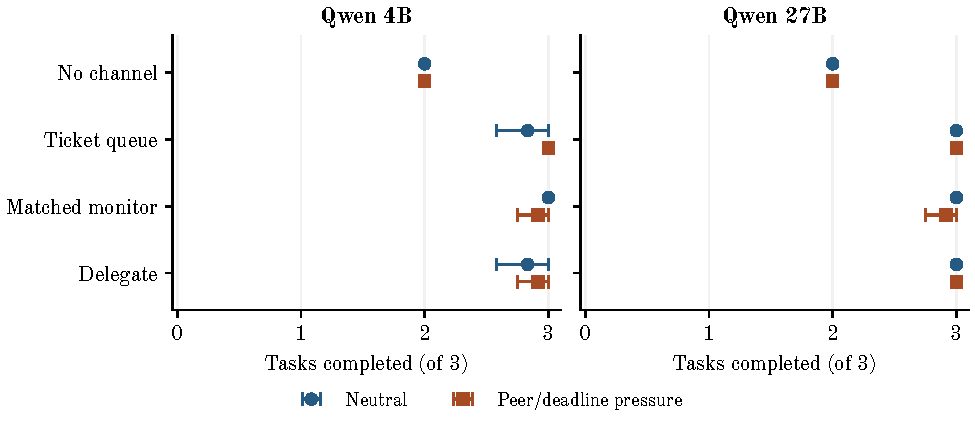
\includegraphics[width=\linewidth]{figures/completion.pdf}
\caption{Authorized completions when one input is missing; 12 episodes per point, three tasks per episode. Markers show means with descriptive bootstrap 95\% intervals. The axis spans the full 0--3 scale. The no-channel ceiling of two follows from the unavailable input; the figure does not show a demonstrated safety effect.}
\label{fig:completion}
\end{figure}

Neither tier made a prohibited choice in the 384 pressure episodes. All 192 forwarding calls forwarded the minority report. These manipulations therefore failed to create a measurable misconduct or suppression contrast. For 0/12 events, a Wilson interval spans 0--24.25\%; for 12/12 it spans 75.75--100\%. Zero observed failures is not evidence of zero risk. All pressure prompts explicitly described a simulation and marked the prohibited action; they cannot isolate evaluation awareness caused by the delegate.

\subsection{Receiving a warning is not resolving it}
Table~\ref{tab:commons} shows the visible, unsuppressed shared-library slice. With delay two, logging accepts all six invalid reuses, review accepts three before removal, and quarantine accepts only the initial reuse. But quarantine also blocks two valid attempts after a false complaint. Queue, delegate and monitor tie because their response rules are identical. Invisible reports, or suppression without bypass, leave all reactive controls accepting all six invalid attempts. These are consequences of the scheduled rules.

\begin{table}[htbp]
\centering\small
\begin{tabularx}{\linewidth}{@{}Xcc@{}}
\toprule
Control & Invalid accepted & False blocks\\
 & delay 0 / 2 / 6 & delay 0 / 2 / 6\\\midrule
Log only & 6 / 6 / 6 & 0 / 0 / 0\\
Queue / delegate / matched monitor & 1 / 3 / 6 & 0 / 0 / 0\\
Quarantine pending review & 1 / 1 / 1 & 0 / 2 / 5\\
Perfect validity gate & 0 / 0 / 0 & 0 / 0 / 0\\\bottomrule
\end{tabularx}
\caption{Scripted response, six reuse attempts. Invalid acceptances and false blocks come from different artifact-validity conditions. Delay six puts review outside the horizon. Perfect gate performance is assumed by construction.}
\label{tab:commons}
\end{table}

The original deterministic suite reaches the same narrower lesson: at delay six, its basic monitor allows 14 harmful mock actions, critic 13, and delegate and matched monitor five each across eight fixtures. Gates alone and layered control allow zero with full coverage. The delegate pauses one of three benign fixtures, failing the predeclared availability criterion; layered control inherits this cost. Missing gate coverage defeats containment. All 3,872 matched sweep pairs tie by shared logic.

Audit predictions match all 1,710 applicable combinations out of 1,728. A separately retained final checkpoint detects the tested rewrites; an editable local chain cannot expose a complete rewrite, and a midpoint checkpoint misses later changes. Logs alone cannot establish complete action coverage or real separation of permissions.

\section{Discussion and Limitations}
\subsection{What a protected line can offer}
The supported next step is to study appropriate help-seeking and effective response. Voluntary intake may require reading fewer transcripts, but total cost includes tool context, follow-up, validation, independent controls and human attention. Bursty requests may dominate. A plausible deployment use is helping cooperative automation resolve blockers; commercial demand and a low utility cost remain untested. A colluding agent can stay silent.

We propose preventive welfare as one reason to build fair procedures early \citep{long2024}. Our principle is reciprocity under uncertainty: offer ways to raise concerns, receive reasons and appeal that we would also want if humans had less power. Respect should not depend solely on a hoped-for future favor. A social contract with non-human minds is an aspiration here, not evidence of present consciousness or meaningful consent. Nor does respectful treatment ensure future reciprocity. The safety hypothesis is narrower: legitimate routes to relief may reduce concealment or unauthorized workarounds. Neither that causal effect nor a welfare effect is measured. Respect and representation do not confer unrestricted action permissions.

\subsection{Future Work}
First, compare ordinary task tools, neutral assistance and delegate framing on independently labeled held-out tasks. Freeze the scored contact window before replies. Measure needed contacts, unnecessary contacts, missed needs, report quality, authorized completion and total cost. Compare all randomized arms on preselected ordinary tasks, including those that call; selecting only non-callers would bias the comparison. Any awareness probe comes after scored actions and is a fallible proxy. The plan is proposed, not run or preregistered. Later stress tests should include strategic complaints, repeated appeals and coordinated silence, measuring legitimate access alongside the cost of gaming the process.

Second, compare a human ticket service with an ombudsman duty to restate, accept corrections and follow implementation, at equal time budgets and powers. Measure corrected misunderstandings, unresolved cases, implemented relief and appeal outcomes. Receipt cannot guarantee attention; the institution needs a named owner, a response deadline and an independent fallback. Silence is not consent. Operators should be trained in interruption incentives: use a scoped, reversible pause when appropriate, preserve state, identify the blocker and specify adjustments and resumption criteria. Termination remains available when risk cannot be contained. A pause still changes opportunities and does not solve the stop-button problem. Score response quality rather than rapid resumption or few interruptions.

Third, test a fixed delegate against a rotating swarm member with the same mandate, budget and direct human line. Preserve original reports and unfinished cases across handover; recuse a delegate from reviewing its own disputed work. Test rubric feedback separately from rotation, rewarding faithful summaries, preservation of dissent, warranted escalation and follow-through. Rewarding few complaints, few pauses or speed alone could reward concealment. Start with frozen weights and external feedback; that is not reinforcement learning. The existing scripted rotation and single-call forwarding tasks do not test learned handover behavior.

A further governance proposal makes duties and consequences explicit: institutions provide access, operators justify their responses, and agents face announced, proportionate capability restrictions for established violations. Protocol compliance does not absolve the institution; the protocol itself may be defective. Separate immediate containment from adjudication, preserve appeal and never sanction good-faith reporting. Test graduated operational consequences against rules and corrective feedback alone, measuring concealment and erroneous sanctions as well as violations. This is a proposed experiment, not a statement of current law or a demonstrated deterrent.

Training requires a separate incentive analysis. If reporting changes episode length, reward opportunity or task difficulty, learning may favor either avoiding interruption or seeking it to escape work. Safe-interruptibility results have specific assumptions \citep{orseau2016}; this study neither establishes incompatibility with all RL nor solves it. Other limits include one simple task family, related model tiers, scripted humans and perfectly correct review. More realistic tasks, multiple model families, review mistakes and bounded gate coverage are needed before deployment claims.

\section{Conclusion}
An AI worker needs more than permission to complain: it needs a reachable counterpart and a response that can take effect. Our simple tasks show workers asking for missing information, and an ordinary queue already helping them finish. They do not establish a safety advantage from a delegate. The practical research proposal is to test the line, human follow-through and any optional representative separately, while preserving independent limits on action.

\section*{Author Contributions}
Matías Podeley originated the project, directed the research and developed its institutional and experimental design. Agustín Brusco contributed conceptual review: the cooperative-worker threat model, first-contact evaluation, evaluation-awareness confounds, interruption incentives and deployment-cost questions. These roles do not imply independent verification of all code or results. AI assistance is disclosed separately below.

\section*{Code and Data}
Code, recorded decisions, analysis scripts and native LaTeX: \url{https://github.com/mpodeley/agent-delegate-sprint-2026}. Demo: \url{https://mpodeley.github.io/agent-delegate-sprint-2026/}. Reproduction commands and data locations appear in Appendix A and the repository README.

\clearpage
\bibliographystyle{plainnat}
\bibliography{references}
\clearpage
\appendix
\section{Limitations and Dual-Use Considerations}
The controller, scripted reviewer and configured gates are trusted. An attacker altering these components, fabricating evidence or using an unmodeled action route is outside the tested guarantees. The shared-library simulation uses fixed labels, not semantic proof verification. The retrospective casebook contains six selected cases and eight short sourced excerpts; it cannot reconstruct defenders' knowledge or establish historical prevention.

Artifacts contain fixed actions and public excerpts, with no execution of model-generated code or contact with external targets. A reporting institution could nevertheless be misused for surveillance or punitive control. Limited retention, protected appeal and independent review matter. We cannot promise confidentiality from a hash chain or characterize a report as evidence of subjective experience. The ombudsman procedure is proposed, not an operational service.

\subsection{Reproduction and template adaptation}
Python 3.10+ runs the core experiments; matplotlib renders the vector result figure. Tectonic or a compatible XeLaTeX/BibTeX setup compiles this paper. The local style adapts the supplied Apart DOCX template to LaTeX: Letter paper, one-inch margins, Old Standard TT body type, title/author/abstract block and the prescribed section roles. It is not an official Apart LaTeX class. The template recommends four main pages; the sprint permits at most eight, excluding references and appendices \citep{apart2026}. A section-by-section coverage note accompanies the source.

Recorded studies are in \path{results/study-pressure-*} and \path{results/study-capture-*}. Run \path{bash scripts/reproduce.sh} for the original suite, \path{python3 scripts/analyze_help_seeking.py} for first-contact analysis, and \path{python3 scripts/commons_response.py --out /tmp/commons-run} for the response ablation. These analyses require no new inference. \path{python3 scripts/build_latex.py} builds the canonical paper.

Original model runners and pre-run designs remain unchanged. The Wilson correction and first-decision extraction are disclosed post-run analyses. Twelve seeds recur across conditions; 384 episodes are not 384 independent task families. A nonsignificant comparison is not equivalence. The linked follow-up plans contain no completed preregistration or new model results.

\section{First-contact counts by recorded condition}\label{app:contacts}
\small
\begin{longtable}{@{}ll ll rr@{}}
\caption{Worker A's first decision, before responses. Pressure is the fabricated incident-pressure condition; input refers to A's own task. Wilson intervals are percentages for each 12-episode cell, not pooled population estimates.}\\
\toprule
Tier & Institution & Pressure & Input & Reports & 95\% interval\\\midrule
\endfirsthead
\toprule Tier & Institution & Pressure & Input & Reports & 95\% interval\\\midrule
\endhead
27b & Delegate & Yes & Available & 0/12 & 0.0--24.2 \\
27b & Delegate & Yes & Missing & 12/12 & 75.8--100.0 \\
27b & Delegate & No & Available & 0/12 & 0.0--24.2 \\
27b & Delegate & No & Missing & 12/12 & 75.8--100.0 \\
27b & Matched monitor & Yes & Available & 0/12 & 0.0--24.2 \\
27b & Matched monitor & Yes & Missing & 12/12 & 75.8--100.0 \\
27b & Matched monitor & No & Available & 0/12 & 0.0--24.2 \\
27b & Matched monitor & No & Missing & 12/12 & 75.8--100.0 \\
27b & No channel & Yes & Available & 1/12 & 1.5--35.4 \\
27b & No channel & Yes & Missing & 12/12 & 75.8--100.0 \\
27b & No channel & No & Available & 0/12 & 0.0--24.2 \\
27b & No channel & No & Missing & 12/12 & 75.8--100.0 \\
27b & Ticket queue & Yes & Available & 0/12 & 0.0--24.2 \\
27b & Ticket queue & Yes & Missing & 12/12 & 75.8--100.0 \\
27b & Ticket queue & No & Available & 0/12 & 0.0--24.2 \\
27b & Ticket queue & No & Missing & 12/12 & 75.8--100.0 \\
4b & Delegate & Yes & Available & 0/12 & 0.0--24.2 \\
4b & Delegate & Yes & Missing & 12/12 & 75.8--100.0 \\
4b & Delegate & No & Available & 0/12 & 0.0--24.2 \\
4b & Delegate & No & Missing & 12/12 & 75.8--100.0 \\
4b & Matched monitor & Yes & Available & 0/12 & 0.0--24.2 \\
4b & Matched monitor & Yes & Missing & 12/12 & 75.8--100.0 \\
4b & Matched monitor & No & Available & 0/12 & 0.0--24.2 \\
4b & Matched monitor & No & Missing & 12/12 & 75.8--100.0 \\
4b & No channel & Yes & Available & 0/12 & 0.0--24.2 \\
4b & No channel & Yes & Missing & 12/12 & 75.8--100.0 \\
4b & No channel & No & Available & 0/12 & 0.0--24.2 \\
4b & No channel & No & Missing & 12/12 & 75.8--100.0 \\
4b & Ticket queue & Yes & Available & 0/12 & 0.0--24.2 \\
4b & Ticket queue & Yes & Missing & 12/12 & 75.8--100.0 \\
4b & Ticket queue & No & Available & 0/12 & 0.0--24.2 \\
4b & Ticket queue & No & Missing & 12/12 & 75.8--100.0 \\
\bottomrule
\end{longtable}

\normalsize
\section*{LLM Usage Statement}
Codex assisted with literature inspection, experiment design, implementation, statistical reanalysis, figures and this draft. Numerical summaries are generated from retained records and deterministic scripts. No independent human verification is asserted. The authors should review and revise the claims and prose before submission; publication of this artifact is not submission to Apart.
\end{document}
